\section{Robot Finger}

\subsection{Prepare Parts for the Robot Finger}

\begin{table}[ht!]
  	\begin{minipage}[b]{0.50\linewidth}\centering
	\scalebox{0.97}{
	\begin{tabular}{ | c | c |}
		\hline
		{\bf{Part}} & {\bf{Qty}}\\ \hline
    		FingerBase1 & 8  \\ \hline
    		FingerBase2 & 4  \\ \hline
    		FingerBase3 & 4  \\ \hline
    		FingerMCP & 4  \\ \hline
    		TubePlateMCP & 8  \\ \hline
		FingerPIP& 4 \\ \hline
		FingerDIP & 4 \\ \hline
		Tubeplate & 12 \\ \hline
    		tubeMCP & 8  \\ \hline
    		tubePIP & 8  \\ \hline
    		tubeDIP & 8  \\ \hline
		M3x12 & 4 \\ \hline
		M3Washer & 16 \\ \hline
		M3Nut & 4 \\ \hline
		pulley & 4 \\ \hline
    	\end{tabular}
	}
	\end{minipage}
	\hspace{0.5cm}	
	\begin{minipage}[b]{0.50\linewidth}\centering
	\scalebox{1}{
	\begin{tabular}{ | c |}
		\hline
 		\multicolumn{1}{|c|}{\bf{Tools}} \\
		\hline
		Acrylic Glue \\ \hline
		Super Glue \\ \hline
		Allen Wrench 2.5mm\\ \hline
		Open-End Wrench \\ \hline
    	\end{tabular}
	}
  	\end{minipage}
\end{table}

\vspace{0.2cm}

\begin{center}
\begin{tikzpicture}
\node [mybox] (box){%
  	\begin{minipage}[b]{0.50\linewidth}\centering
	\begin{tabular}{ c }
		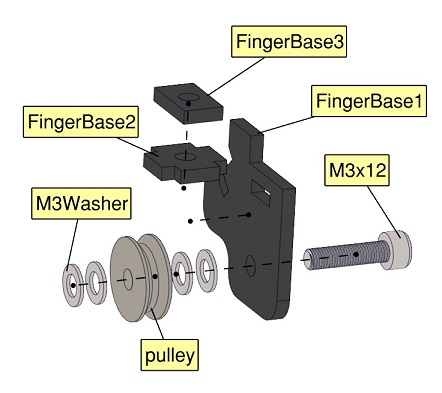
\includegraphics[width=6cm]{figures/Finger/Finger1.jpg}
    	\end{tabular}
	\end{minipage}
	\hspace{0.5cm}	
	\begin{minipage}[b]{0.50\linewidth}
	\begin{tabular}{ l }
		     \Circled{1} Glue FingerBase2 and FingerBase3 together \\ using acrylic glue. \\
		     \Circled{2} Glue FingerBase1 and FingerBase2-3 together \\ using acrylic glue. \\
		     \Circled{3} Continue as you see in the picture. \\
		     \Circled{!} Pay attention not to forget the M3 washers.
    	\end{tabular}
  	\end{minipage}
};
\node[mytitle, right=10pt] at (box.north west) {6.1.1};
\end{tikzpicture}%
\end{center}

\newpage

\begin{center}
\begin{tikzpicture}
\node [mybox] (box){%
  	\begin{minipage}[b]{0.50\linewidth}\centering
	\begin{tabular}{ c }
           	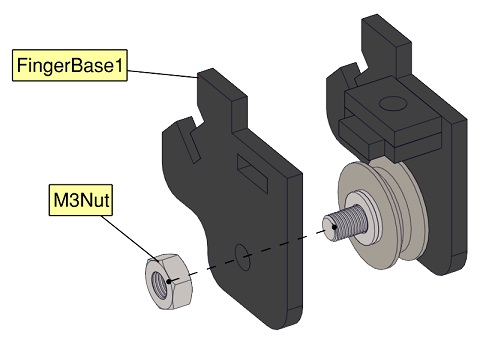
\includegraphics[width=6cm]{figures/Finger/Finger2.jpg}
    	\end{tabular}
	\end{minipage}
	\hspace{0.5cm}	
	\begin{minipage}[b]{0.50\linewidth}
	\begin{tabular}{ l }
		\Circled{1} Attach FingerBase1 to the previous part.\\  
		\Circled{2} Glue the previous part and FingerBase1 \\ together using acrylic glue. \\
		\Circled{3} Screw the M3Nut to the M3x12 screw.\\
		\Circled{!}  M3 washers must be in the right position. \\  
		\Circled{!}  Tighten the screw until the pulley\\ can freely move. 
    	\end{tabular}
  	\end{minipage}
};
\node[mytitle, right=10pt] at (box.north west) {6.1.2};
\end{tikzpicture}%
\end{center}

\vspace{0.2cm}

\begin{center}
\begin{tikzpicture}
\node [mybox] (box){%
  	\begin{minipage}[b]{0.50\linewidth}\centering
	\begin{tabular}{ l }
		\Circled{1} Glue FingerMCP and TubePlateMCP parts \\ together, using acrylic glue. \\
    	\end{tabular}
	\end{minipage}
	\hspace{0.5cm}	
	\begin{minipage}[b]{0.50\linewidth}
	\begin{tabular}{ c }
		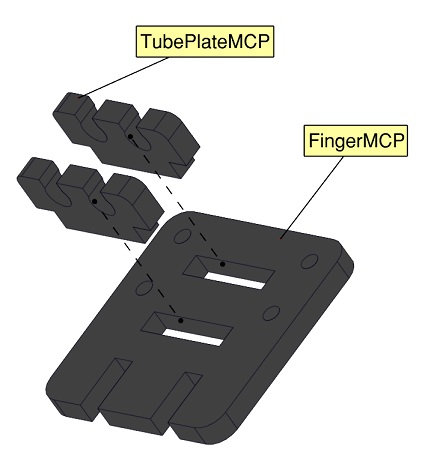
\includegraphics[width=6cm]{figures/Finger/Finger3.jpg}
    	\end{tabular}
  	\end{minipage}
};
\node[mytitle, right=10pt] at (box.north west) {6.1.3};
\end{tikzpicture}%
\end{center}

\vspace{0.2cm}

\begin{center}
\begin{tikzpicture}
\node [mybox] (box){%
  	\begin{minipage}[b]{0.50\linewidth}\centering
	\begin{tabular}{ c }
		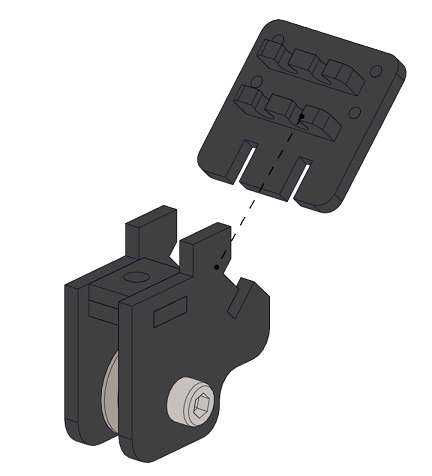
\includegraphics[width=6cm]{figures/Finger/Finger4.jpg}
    	\end{tabular}
	\end{minipage}
	\hspace{0.5cm}	
	\begin{minipage}[b]{0.50\linewidth}
	\begin{tabular}{ l }
		\Circled{1} Attach the FingerMCP part\\ to the FingerBase1 slots. \\ 
		\Circled{!} The FingerMCP part must fit\\ into the FingerBase1 slots. \\
		\Circled{2} Glue the two parts together\\ with acrylic glue.
    	\end{tabular}
  	\end{minipage}
};
\node[mytitle, right=10pt] at (box.north west) {6.1.4};
\end{tikzpicture}%
\end{center}

\newpage

\begin{center}
\begin{tikzpicture}
\node [mybox] (box){%
  	\begin{minipage}[b]{0.50\linewidth}\centering
	\begin{tabular}{ l }
		\Circled{1} Insert the low friction tubes to the \\ tube plates, as you see in the picture. \\
		\Circled{2} Glue the edges of the tubes to the \\ tube plate, using super glue. 
    	\end{tabular}
	\end{minipage}
	\hspace{0.5cm}	
	\begin{minipage}[b]{0.50\linewidth}
	\begin{tabular}{ l }
		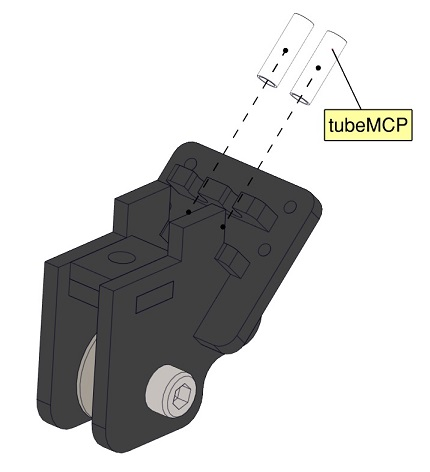
\includegraphics[width=6cm]{figures/Finger/Finger5.jpg}
    	\end{tabular}
  	\end{minipage}
};
\node[mytitle, right=10pt] at (box.north west) {6.1.5};
\end{tikzpicture}%
\end{center}

\vspace{0.2cm}

\begin{center}
\begin{tikzpicture}
\node [mybox] (box){%
	\begin{tabular}{ c }
           	     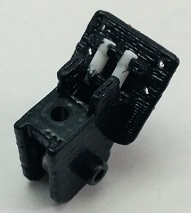
\includegraphics[width = 4cm]{figures/Finger/Finger6.jpg}
    	\end{tabular}
};
\node[mytitle, right=10pt] at (box.north west) {FingerBase part};
\end{tikzpicture}%
\end{center}

\vspace{0.2cm}

\begin{center}
\begin{tikzpicture}
\node [mybox] (box){%
  	\begin{minipage}[b]{0.50\linewidth}\centering
	\begin{tabular}{ l }
		\Circled{1} Glue FingerPIP and TubePlate together,\\ using acrylic glue. \\
    	\end{tabular}
	\end{minipage}
	\hspace{0.5cm}	
	\begin{minipage}[b]{0.50\linewidth}
	\begin{tabular}{ c }
		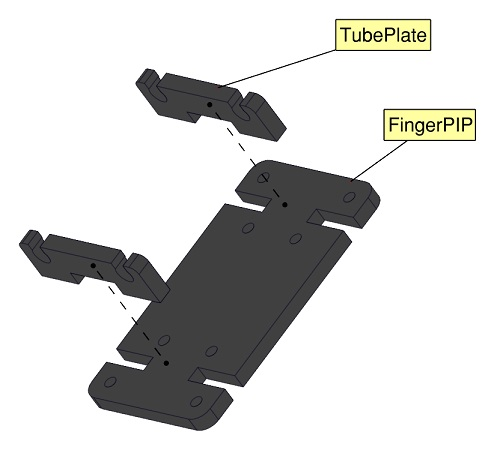
\includegraphics[width=6cm]{figures/Finger/Finger7.jpg}
    	\end{tabular}
  	\end{minipage}
};
\node[mytitle, right=10pt] at (box.north west) {6.1.6};
\end{tikzpicture}%
\end{center}

\newpage

\begin{center}
\begin{tikzpicture}
\node [mybox] (box){%
  	\begin{minipage}[b]{0.50\linewidth}\centering
	\begin{tabular}{ l }
		\Circled{1} Insert the low friction tubes to the \\ tube plates, as you see in the picture. \\
		\Circled{2} Glue the edges of the tubes to the \\ tube plate, using super glue. 
    	\end{tabular}
	\end{minipage}
	\hspace{0.5cm}	
	\begin{minipage}[b]{0.50\linewidth}
	\begin{tabular}{ l }
		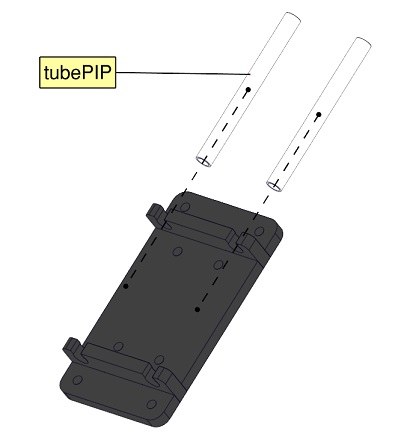
\includegraphics[width=6cm]{figures/Finger/Finger8.jpg}
    	\end{tabular}
  	\end{minipage}
};
\node[mytitle, right=10pt] at (box.north west) {6.1.7};
\end{tikzpicture}%
\end{center}

\vspace{0.2cm}

\begin{center}
\begin{tikzpicture}
\node [mybox] (box){%
  	\begin{minipage}[b]{0.50\linewidth}\centering
	\begin{tabular}{ c }
		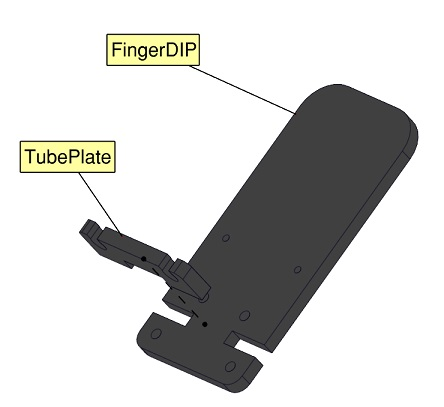
\includegraphics[width=6cm]{figures/Finger/Finger9.jpg}
    	\end{tabular}
	\end{minipage}
	\hspace{0.5cm}	
	\begin{minipage}[b]{0.50\linewidth}
	\begin{tabular}{ l }
		\Circled{1} Glue FingerDIP and TubePlate together,\\ using acrylic glue. \\
    	\end{tabular}
  	\end{minipage}
};
\node[mytitle, right=10pt] at (box.north west) {6.1.8};
\end{tikzpicture}%
\end{center}

\vspace{0.2cm}

\begin{center}
\begin{tikzpicture}
\node [mybox] (box){%
  	\begin{minipage}[b]{0.50\linewidth}\centering
	\begin{tabular}{ l }
		\Circled{1} Insert the low friction tubes to the \\ tube plates, as you see in the picture. \\
		\Circled{2} Glue the edges of the tubes to the \\ tube plate, using super glue.
    	\end{tabular}
	\end{minipage}
	\hspace{0.5cm}	
	\begin{minipage}[b]{0.50\linewidth}
	\begin{tabular}{ l }
		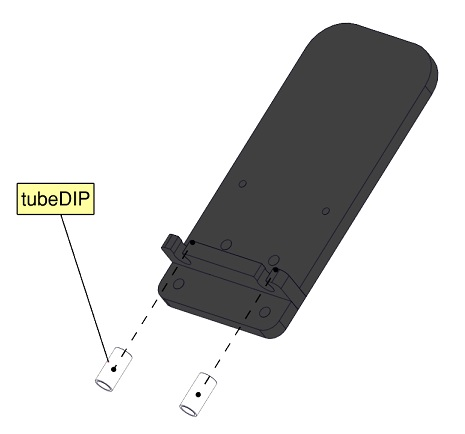
\includegraphics[width=6cm]{figures/Finger/Finger10.jpg}
    	\end{tabular}
  	\end{minipage}
};
\node[mytitle, right=10pt] at (box.north west) {6.1.9};
\end{tikzpicture}%
\end{center}

\newpage

\begin{center}
\begin{tikzpicture}
\node [mybox] (box){%
  	\begin{minipage}[b]{0.50\linewidth}\centering
	\begin{tabular}{ c }
		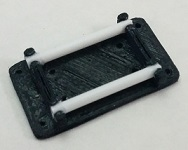
\includegraphics[width = 4.8cm]{figures/Finger/Finger11.jpg}
    	\end{tabular}
	\end{minipage}
	\hspace{0.5cm}	
	\begin{minipage}[b]{0.50\linewidth}
	\begin{tabular}{ c }
		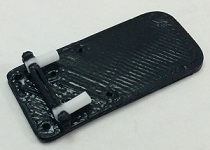
\includegraphics[width = 5.2cm]{figures/Finger/Finger12.jpg}
    	\end{tabular}
  	\end{minipage}
};
\node[mytitle, right=10pt] at (box.north west) {FingerPIP and FingerDIP parts};
\end{tikzpicture}%
\end{center}

\vspace{0.2cm}

\subsection{Stitching the Rigid Parts onto the Flexure Joints }
\begin{table}[ht!]
  	\begin{minipage}[b]{0.50\linewidth}\centering
	\scalebox{0.97}{
	\begin{tabular}{ | c | c |}
		\hline
		{\bf{Part}} & {\bf{Qty}}\\ \hline
    		FingerBase & 4  \\ \hline
    		FingerPIP & 4  \\ \hline
    		FingerDIP & 4  \\ \hline
    		Joint1 & 4  \\ \hline
    		Joint2 & 4  \\ \hline
    	\end{tabular}
	}
	\end{minipage}
	\hspace{0.5cm}	
	\begin{minipage}[b]{0.50\linewidth}\centering
	\scalebox{1}{
	\begin{tabular}{ | c |}
		\hline
 		\multicolumn{1}{|c|}{{\bf{Tools}}} \\
		\hline
		Long Darners \\ \hline
		Nylon Fishing Line \\ \hline
		Cutter \\ \hline
		Long-Nose Pliers with Side-Cutting \\ \hline
		Precision Ruler \\ \hline
		Scissors \\ \hline
    	\end{tabular}
	}
  	\end{minipage}

\end{table}

\vspace{0.2cm}

\begin{center}
	\begin{tabular}{ c c }
		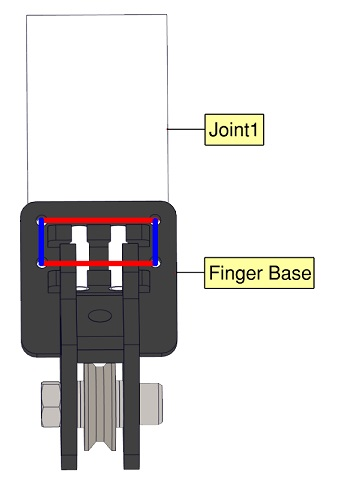
\includegraphics[width=4cm]{figures/Finger/Finger13.jpg} &
		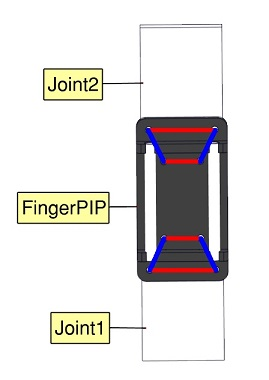
\includegraphics[width=4cm]{figures/Finger/Finger14.jpg}
    	\end{tabular}
\end{center}

\vspace{0.5cm}	

In order to connect together the rigid parts that we assembled in the previous sections, we use silicone sheets as flexure joints. 
These silicone sheets can be stitched onto the rigid parts, following the pattern that you see in the picture.
This sewing pattern creates a rigid connection between the rigid part and the flexure joint. \\
We use nylon fishing line and long darners for sewing. In the picture, the red lines depict a fishing line
passing from both sides of the rigid part and the flexure joint, while the blue lines depict a fishing line that passes only from 
the lower side of the flexure joint. The same sewing pattern can be used for both fingerPIP and fingerDIP parts. The following steps explain exactly this process.
	
\newpage

\begin{center}
\begin{tikzpicture}
\node [mybox] (box){%
  	\begin{minipage}[b]{0.50\linewidth}\centering
	\begin{tabular}{ c }
		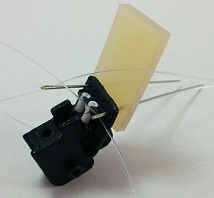
\includegraphics[width=6cm]{figures/Finger/Finger15.jpg} 
    	\end{tabular}
	\end{minipage}
	\hspace{0.5cm}	
	\begin{minipage}[b]{0.50\linewidth}
	\begin{tabular}{ l }
		\Circled{1} Cut a 450mm fishing line. \\
		\Circled{2} Insert the fishing line to the holes \\ of two long darners. \\
		\Circled{3} Insert from the outer holes of the \\ upper side of the fingerMCP part the two \\  long darners, as you see in the picture. \\
    	\end{tabular}
  	\end{minipage}
};
\node[mytitle, right=10pt] at (box.north west) {6.2.1};
\end{tikzpicture}%
\end{center}

\vspace{0.2cm}

\begin{center}
\begin{tikzpicture}
\node [mybox] (box){%
  	\begin{minipage}[b]{0.50\linewidth}\centering
	\begin{tabular}{ l }
		\Circled{1} Insert each of the darners, to the hole \\ of the other darner. \\
		\Circled{2} Repeat \Circled{1} 2 times. \\
		\Circled{!} The darners are now in the lower side of \\ the fingerMCP part.\\
		\Circled{3} Insert the darners to the inner holes \\ of the fingerMCP part. \\
    	\end{tabular}
	\end{minipage}
	\hspace{0.5cm}	
	\begin{minipage}[b]{0.50\linewidth}
	\begin{tabular}{ l }
		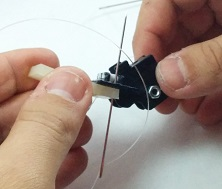
\includegraphics[width=6cm]{figures/Finger/Finger16.jpg}
    	\end{tabular}
  	\end{minipage}
};
\node[mytitle, right=10pt] at (box.north west) {6.2.2};
\end{tikzpicture}%
\end{center}

\vspace{0.2cm}

\begin{center}
\begin{tikzpicture}
\node [mybox] (box){%
  	\begin{minipage}[b]{0.50\linewidth}\centering
	\begin{tabular}{ c }
           	     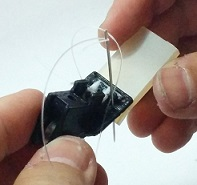
\includegraphics[width=6cm]{figures/Finger/Finger17.jpg} 
    	\end{tabular}
	\end{minipage}
	\hspace{0.5cm}	
	\begin{minipage}[b]{0.50\linewidth}
	\begin{tabular}{ l }
		\Circled{1} Insert each one of the darners to the hole \\ of the other darner.\\
		\Circled{2} Repeat \Circled{1} 3 times. \\
		\Circled{!} The darners are now in the lower side of \\ the fingerMCP part.
    	\end{tabular}
  	\end{minipage}
};
\node[mytitle, right=10pt] at (box.north west) {6.2.3};
\end{tikzpicture}%
\end{center}

\newpage

\begin{center}
\begin{tikzpicture}
\node [mybox] (box){%
  	\begin{minipage}[b]{0.50\linewidth}\centering
	\begin{tabular}{ l }
		\Circled{1} Remove the darners from the fishing line. \\
		\Circled{2} With the two ends of the fishing line do \\ multiple surgeon's knots.
    	\end{tabular}
	\end{minipage}
	\hspace{0.5cm}	
	\begin{minipage}[b]{0.50\linewidth}
	\begin{tabular}{ c }
		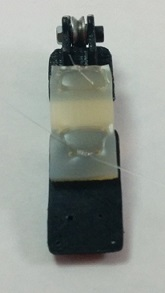
\includegraphics[width=3cm]{figures/Finger/Finger18.jpg}
    	\end{tabular}
  	\end{minipage}
};
\node[mytitle, right=10pt] at (box.north west) {6.2.4};
\end{tikzpicture}%
\end{center}

\vspace{0.2cm}

\begin{center}
\begin{tikzpicture}
\node [mybox] (box){%
  	\begin{minipage}[b]{0.50\linewidth}\centering
	\begin{tabular}{ c }
           	     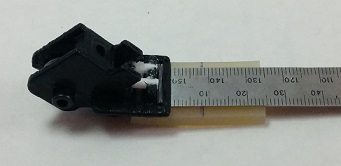
\includegraphics[width=6cm]{figures/Finger/Finger19.jpg}
    	\end{tabular}
	\end{minipage}
	\hspace{0.5cm}	
	\begin{minipage}[b]{0.50\linewidth}
	\begin{tabular}{ l }
		\Circled{1} Use a ruler to measure 8mm from the edge \\ of the fingerMCP part and draw a line\\ with a pen.
    	\end{tabular}
  	\end{minipage}
};
\node[mytitle, right=10pt] at (box.north west) {6.2.5};
\end{tikzpicture}%
\end{center}

\vspace{0.2cm}

\begin{center}
\begin{tikzpicture}
\node [mybox] (box){%
  	\begin{minipage}[b]{0.50\linewidth}\centering
	\begin{tabular}{ l }
		\Circled{1} Cut a 450mm fishing line. \\
		\Circled{2} Insert the fishing line to the holes \\ of two long darners. \\
		\Circled{3} Center the fingerPIP part with the silicone part\\ and align it with the line from the previous step.\\
		\Circled{4} Insert from the outer holes of the lower side \\ of the fingerPIP part the two long darners, \\ as you see in the picture. \\
    	\end{tabular}
	\end{minipage}
	\hspace{0.5cm}	
	\begin{minipage}[b]{0.50\linewidth}
	\begin{tabular}{ c }
		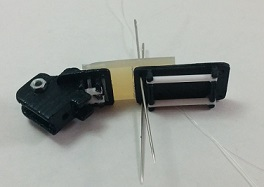
\includegraphics[width=6cm]{figures/Finger/Finger20.jpg} 
    	\end{tabular}
  	\end{minipage}
};
\node[mytitle, right=10pt] at (box.north west) {6.2.6};
\end{tikzpicture}%
\end{center}

\newpage

\begin{center}
\begin{tikzpicture}
\node [mybox] (box){%
  	\begin{minipage}[b]{0.50\linewidth}\centering
	\begin{tabular}{ c }
		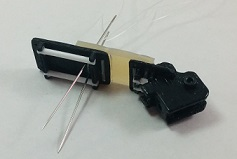
\includegraphics[width=6cm]{figures/Finger/Finger21.jpg}
    	\end{tabular}
	\end{minipage}
	\hspace{0.5cm}	
	\begin{minipage}[b]{0.50\linewidth}
	\begin{tabular}{ l }
		\Circled{1} Insert each one of the darners to the hole of \\ the other darner.\\
		\Circled{2} Repeat \Circled{1} for 3 times. \\
		\Circled{!} The darners are now in the lower side \\ of the fingerPIP part. 
    	\end{tabular}
  	\end{minipage}
};
\node[mytitle, right=10pt] at (box.north west) {6.2.7};
\end{tikzpicture}%
\end{center}

\vspace{0.2cm}

\begin{center}
\begin{tikzpicture}
\node [mybox] (box){%
  	\begin{minipage}[b]{0.50\linewidth}\centering
	\begin{tabular}{ l }
		\Circled{1} Insert the darners to the inner holes \\ of the fingerPIP part from the lower side.\\
		\Circled{2} Insert each one of the darners to the hole\\ of the other darner.\\
		\Circled{3} Repeat \Circled{2} 3 times.\\
		\Circled{!} The darners are now in the lower side of \\ the fingerPIP part. \\
		\Circled{4} Remove the darners from the fishing line. \\
		\Circled{5} With the two ends of the fishing line do \\ multiple surgeon's knots.\\
    	\end{tabular}
	\end{minipage}
	\hspace{0.5cm}	
	\begin{minipage}[b]{0.50\linewidth}
	\begin{tabular}{ c }
		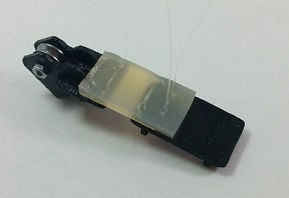
\includegraphics[width=6cm]{figures/Finger/Finger22.jpg}
    	\end{tabular}
  	\end{minipage}
};
\node[mytitle, right=10pt] at (box.north west) {6.2.8};
\end{tikzpicture}%
\end{center}

\vspace{0.2cm}

\begin{center}
\begin{tikzpicture}
\node [mybox] (box){%
  	\begin{minipage}[b]{0.50\linewidth}\centering
	\begin{tabular}{ c }
		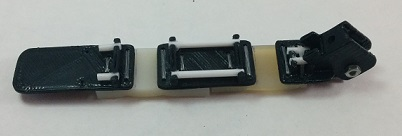
\includegraphics[width=8cm]{figures/Finger/Finger23.jpg}
    	\end{tabular}
	\end{minipage}
	\hspace{0.5cm}	
	\begin{minipage}[b]{0.50\linewidth}
	\begin{tabular}{ l }
		\Circled{1} Repeat the 6.2.6 - 6.2.8 steps for the\\ FingerDIP part. \\
		\Circled{!} Congratulations, now you have a robot finger!
    	\end{tabular}
  	\end{minipage}
};
\node[mytitle, right=10pt] at (box.north west) {Robot Finger};
\end{tikzpicture}%
\end{center}

\newpage

\subsection{Tendon Routing of the Robot Finger}
\begin{table}[ht!]
  	\begin{minipage}[b]{0.50\linewidth}\centering
	\scalebox{0.97}{
	\begin{tabular}{ | c | c |}
		\hline
		{\bf{Part}} & {\bf{Qty}}\\ \hline
    		Robot Finger & 4  \\ \hline
		Dyneema & -- \\ \hline

    	\end{tabular}
	}
	\end{minipage}
	\hspace{0.5cm}	
	\begin{minipage}[b]{0.50\linewidth}\centering
	\scalebox{1}{
	\begin{tabular}{ | c |}
		\hline
 		\multicolumn{1}{|c|}{{\bf{Tools}}} \\
		\hline
		Scissors \\ \hline
		Precision Ruler \\ \hline
    	\end{tabular}
	}
  	\end{minipage}

\end{table}

\vspace{0.2cm}

\begin{center}
\begin{tikzpicture}
\node [mybox] (box){%
  	\begin{minipage}[b]{0.50\linewidth}\centering
	\begin{tabular}{ c }
		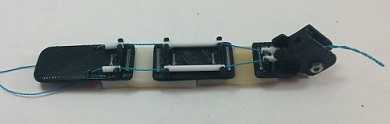
\includegraphics[width=7.5cm]{figures/Finger/Finger24.jpg}
    	\end{tabular}
	\end{minipage}
	\hspace{0.5cm}	
	\begin{minipage}[b]{0.50\linewidth}
	\begin{tabular}{ l }
		\Circled{1} Cut 600mm of the Dyneema fishing line. \\
		\Circled{2} Insert the Dyneema into the low friction tubes\\ starting from the tubeMCP. \\
    	\end{tabular}
  	\end{minipage}
};
\node[mytitle, right=10pt] at (box.north west) {6.3.1};
\end{tikzpicture}%
\end{center}

\vspace{0.2cm}

\begin{center}
\begin{tikzpicture}
\node [mybox] (box){%
  	\begin{minipage}[b]{0.50\linewidth}\centering
	\begin{tabular}{ l }
		\Circled{!}  Now the two edges of the Dyneema are \\ at the end of the tubeMCP. \\
		\Circled{1} Use a M3 spacer of 10mm length as \\ depicted in the picture. \\
    	\end{tabular}
	\end{minipage}
	\hspace{0.5cm}	
	\begin{minipage}[b]{0.50\linewidth}
	\begin{tabular}{ l }
           	     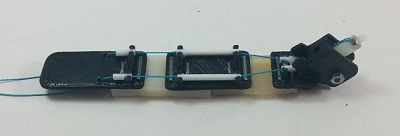
\includegraphics[width=7.5cm]{figures/Finger/Finger25.jpg}
    	\end{tabular}
  	\end{minipage}
};
\node[mytitle, right=10pt] at (box.north west) {6.3.2};
\end{tikzpicture}%
\end{center}

\vspace{0.2cm}

\begin{center}
\begin{tikzpicture}
\node [mybox] (box){%
  	\begin{minipage}[b]{0.50\linewidth}\centering
	\begin{tabular}{ c }
           	     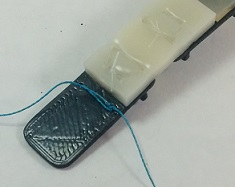
\includegraphics[width=7cm]{figures/Finger/Finger26.jpg}
    	\end{tabular}
	\end{minipage}
	\hspace{0.5cm}	
	\begin{minipage}[b]{0.50\linewidth}
	\begin{tabular}{ l }
		\Circled{1} With the two edges of the Dyneema do \\ multiple surgeon's knots. \\
    	\end{tabular}
  	\end{minipage}
};
\node[mytitle, right=10pt] at (box.north west) {6.3.3};
\end{tikzpicture}%
\end{center}

\newpage

\subsection{Install Soft Fingetips}

\begin{table}[ht!]
  	\begin{minipage}[b]{0.50\linewidth}\centering
	\scalebox{0.97}{
	\begin{tabular}{ | c | c |}
		\hline
		{\bf{Part}} & {\bf{Qty}}\\ \hline
    		Robot Finger &  4  \\ \hline
		Sponge Tape & -- \\ \hline
		Self-adhesive Tape & -- \\ \hline
		Anti-Slip Tape & -- \\ \hline
    	\end{tabular}
	}
	\end{minipage}
	\hspace{0.5cm}	
	\begin{minipage}[b]{0.50\linewidth}\centering
	\scalebox{1}{
	\begin{tabular}{ | c |}
		\hline
 		\multicolumn{1}{|c|}{{\bf{Tools}}} \\
		\hline
		Scissors \\ \hline
    	\end{tabular}
	}
  	\end{minipage}

\end{table}

\vspace{0.2cm}

\begin{center}
\begin{tikzpicture}
\node [mybox] (box){%
  	\begin{minipage}[b]{0.50\linewidth}\centering
	\begin{tabular}{ c }
		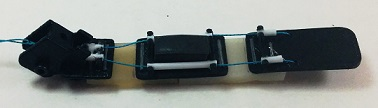
\includegraphics[width=7cm]{figures/Finger/Finger28.jpg}
    	\end{tabular}
	\end{minipage}
	\hspace{0.5cm}	
	\begin{minipage}[b]{0.50\linewidth}
	\begin{tabular}{ l }
		\Circled{1} Cut two pieces of 24mm sponge tape. \\
		\Circled{2} Set the two pieces onto the FingerPIP part. \\
    	\end{tabular}
  	\end{minipage}
};
\node[mytitle, right=10pt] at (box.north west) {6.4.1};
\end{tikzpicture}%
\end{center}

\vspace{0.2cm}

\begin{center}
\begin{tikzpicture}
\node [mybox] (box){%
  	\begin{minipage}[b]{0.50\linewidth}\centering
	\begin{tabular}{ l }
		\Circled{1} Cut a piece of 130mm self-adhesive tape. \\
		\Circled{2} Wrap the tape around the FingerPIP part. \\
    	\end{tabular}
	\end{minipage}
	\hspace{0.5cm}	
	\begin{minipage}[b]{0.50\linewidth}
	\begin{tabular}{ c }
		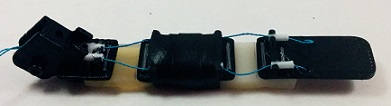
\includegraphics[width=7cm]{figures/Finger/Finger29.jpg}
    	\end{tabular}
  	\end{minipage}
};
\node[mytitle, right=10pt] at (box.north west) {6.4.2};
\end{tikzpicture}%
\end{center}

\vspace{0.2cm}

\begin{center}
\begin{tikzpicture}
\node [mybox] (box){%
  	\begin{minipage}[b]{0.50\linewidth}\centering
	\begin{tabular}{ c }
		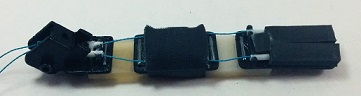
\includegraphics[width=7cm]{figures/Finger/Finger31.jpg}
    	\end{tabular}
	\end{minipage}
	\hspace{0.5cm}	
	\begin{minipage}[b]{0.50\linewidth}
	\begin{tabular}{ l }
		\Circled{1} Cut two pieces of 32mm sponge tape. \\
		\Circled{2} Set the two pieces onto the FingerDIP part. \\
		\Circled{3} Cut a piece of 10mm sponge tape. \\
		\Circled{4} Set the sponge tape onto the empty space \\ of the FingerDIP part. \\
		\Circled{5} Cut two pieces of 40mm sponge tape and \\ set them onto the other side.
    	\end{tabular}
  	\end{minipage}
};
\node[mytitle, right=10pt] at (box.north west) {6.4.3};
\end{tikzpicture}%
\end{center}

\vspace{0.2cm}

\begin{center}
\begin{tikzpicture}
\node [mybox] (box){%
  	\begin{minipage}[b]{0.50\linewidth}\centering
	\begin{tabular}{ c }
		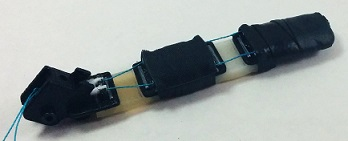
\includegraphics[width=7cm]{figures/Finger/Finger32.jpg}
    	\end{tabular}
	\end{minipage}
	\hspace{0.5cm}	
	\begin{minipage}[b]{0.50\linewidth}
	\begin{tabular}{ l }
		\Circled{1} Cut a piece of 200mm self-adhesive tape. \\
		\Circled{2} Wrap the tape around the FingerDIP part. \\
    	\end{tabular}
  	\end{minipage}
};
\node[mytitle, right=10pt] at (box.north west) {6.4.4};
\end{tikzpicture}%
\end{center}

\newpage

\begin{center}
\begin{tikzpicture}
\node [mybox] (box){%
  	\begin{minipage}[b]{0.50\linewidth}\centering
	\begin{tabular}{ l }
		\Circled{1} Cut a piece of 27mm anti-slip tape. \\
		\Circled{2} Attach the tape onto the FingerPIP part. \\
		\Circled{3} Cut a piece of 40mm anti-slip tape. \\
		\Circled{4} Attach the tape onto the FingerDIP part. \\
		\Circled{!} Cut the edges of the tape at the FingerDIP part. \\
    	\end{tabular}
	\end{minipage}
	\hspace{0.5cm}	
	\begin{minipage}[b]{0.50\linewidth}
	\begin{tabular}{ c }
		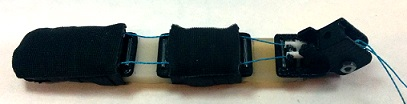
\includegraphics[width=7cm]{figures/Finger/Finger33.jpg}
    	\end{tabular}
  	\end{minipage}
};
\node[mytitle, right=10pt] at (box.north west) {6.4.5};
\end{tikzpicture}%
\end{center}

\vspace{0.5cm}

\subsection{Install Soft Pad to the Top Plate of the Robot Base}

\begin{table}[ht!]
  	\begin{minipage}[b]{0.50\linewidth}\centering
	\scalebox{0.97}{
	\begin{tabular}{ | c | c |}
		\hline
		{\bf{Part}} & {\bf{Qty}}\\ \hline
    		TopPlate & 2  \\ \hline
		Sponge Tape & -- \\ \hline
		Anti-Slip Tape & -- \\ \hline
    	\end{tabular}
	}
	\end{minipage}
	\hspace{0.5cm}	
	\begin{minipage}[b]{0.50\linewidth}\centering
	\scalebox{1}{
	\begin{tabular}{ | c |}
		\hline
 		\multicolumn{1}{|c|}{Tools} \\
		\hline
		Acrylic Glue \\ \hline
		Scissors \\ \hline
    	\end{tabular}
	}
  	\end{minipage}

\end{table}

\vspace{0.2cm}

\begin{center}
\begin{tikzpicture}
\node [mybox] (box){%
  	\begin{minipage}[b]{0.50\linewidth}\centering
	\begin{tabular}{ c }
		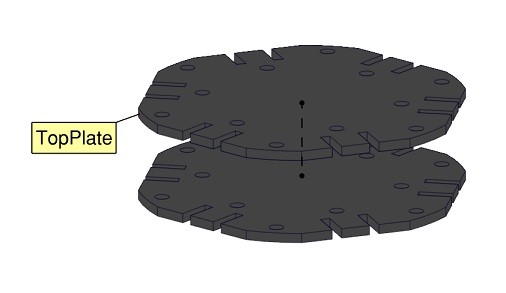
\includegraphics[width=6cm]{figures/Finger/TopPlate1.jpg} 
    	\end{tabular}
	\end{minipage}
	\hspace{0.5cm}	
	\begin{minipage}[b]{0.50\linewidth}
	\begin{tabular}{ l }
		\Circled{1} Glue the TopPlate parts. \\
		\Circled{!} Center the two parts as depicted.
    	\end{tabular}
  	\end{minipage}
};
\node[mytitle, right=10pt] at (box.north west) {6.5.1};
\end{tikzpicture}%
\end{center}

\vspace{0.2cm}

\begin{center}
\begin{tikzpicture}
\node [mybox] (box){%
  	\begin{minipage}[b]{0.50\linewidth}\centering
	\begin{tabular}{ l }
		\Circled{1} Cut three pieces of 25mm sponge tape. \\
		\Circled{2} Put the pieces of tape in the middle of \\ the TopPlate part. \\
    	\end{tabular}
	\end{minipage}
	\hspace{0.5cm}	
	\begin{minipage}[b]{0.50\linewidth}
	\begin{tabular}{ c }
		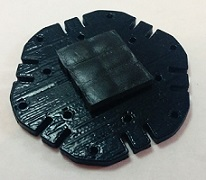
\includegraphics[width=6cm]{figures/Finger/TopPlate2.jpg} 
    	\end{tabular}
  	\end{minipage}
};
\node[mytitle, right=10pt] at (box.north west) {6.5.2};
\end{tikzpicture}%
\end{center}

\newpage

\begin{center}
\begin{tikzpicture}
\node [mybox] (box){%
  	\begin{minipage}[b]{0.50\linewidth}\centering
	\begin{tabular}{ c }
		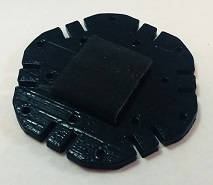
\includegraphics[width=5.5cm]{figures/Finger/TopPlate3.jpg} 
    	\end{tabular}
	\end{minipage}
	\hspace{0.5cm}	
	\begin{minipage}[b]{0.50\linewidth}
	\begin{tabular}{ l }
		\Circled{1} Cut a piece of 32mm anti-slip tape. \\
		\Circled{2} Attach the tape pieces onto the sponge tape. \\
    	\end{tabular}
  	\end{minipage}
};
\node[mytitle, right=10pt] at (box.north west) {6.5.3};
\end{tikzpicture}%
\end{center}

\vspace{0.5cm}

\subsection{Install the Robot Fingers to the TopPlate}

\begin{table}[ht!]
  	\begin{minipage}[b]{0.50\linewidth}\centering
	\scalebox{0.97}{
	\begin{tabular}{ | c | c |}
		\hline
		{\bf{Part}} & {\bf{Qty}}\\ \hline
    		TopPlate & 1 \\ \hline
		Robot Finger & 4 \\ \hline
		M3x12 & 4 \\ \hline
		M3Washer & 4 \\ \hline
		M3Nut & 5 \\ \hline
    	\end{tabular}
	}
	\end{minipage}
	\hspace{0.5cm}	
	\begin{minipage}[b]{0.50\linewidth}\centering
	\scalebox{1}{
	\begin{tabular}{ | c |}
		\hline
 		\multicolumn{1}{|c|}{{\bf{Tools}}} \\
		\hline
		Allen Wrench 2.5mm \\ \hline
    	\end{tabular}
	}
  	\end{minipage}

\end{table}

\vspace{0.2cm}

\begin{center}
\begin{tikzpicture}
\node [mybox] (box){%
  	\begin{minipage}[b]{0.50\linewidth}\centering
	\begin{tabular}{ c }
		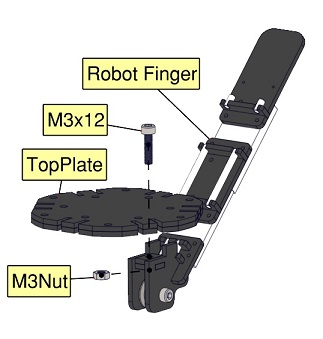
\includegraphics[width=6cm]{figures/Finger/TopPlate4.jpg}
    	\end{tabular}
	\end{minipage}
	\hspace{0.5cm}	
	\begin{minipage}[b]{0.50\linewidth}
	\begin{tabular}{ l }
		\Circled{1} Keep the TopPlate part and the robot finger.\\
		\Circled{2} Insert the M3Nut in the FingerBase part.\\
		\Circled{3} Insert the robot finger to the slot \\ of the TopPlate.\\
		\Circled{4} Center the M3Nut with the holes of \\ the FingerBase and the TopPlate parts.\\
		\Circled{5} Insert the M3x12 screw with the M3 washer \\ in the hole of the TopPlate.\\
		\Circled{6} Tighten the M3x12 screw. \\
		\Circled{7} Repeat the steps to install all the robot \\ fingers to the TopPlate.
    	\end{tabular}
  	\end{minipage}
};
\node[mytitle, right=10pt] at (box.north west) {6.6.1};
\end{tikzpicture}%
\end{center}

\newpage

\begin{center}
\begin{tikzpicture}
\node [mybox] (box){%
	\begin{tabular}{ c }
		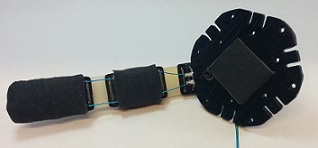
\includegraphics[width=7cm]{figures/Finger/TopPlate5.jpg}
    	\end{tabular}
};
\node[mytitle, right=10pt] at (box.north west) {TopPlate with Robot Finger};
\end{tikzpicture}%
\end{center}

\vspace{0.1cm}

\begin{center}
\begin{tikzpicture}
\node [mybox] (box){%
  	\begin{minipage}[b]{0.50\linewidth}\centering
	\begin{tabular}{ l }
		\Circled{1} Cut 20mm of Dyneema fishing line.\\
		\Circled{2} Pass the Dyneema fishing line through\\ the FingerBase tendon loop or spacer. \\
                \Circled{!} Leave both edges of the Dyneema free!\\
		\Circled{3} Repeat the steps for all robot fingers. \\ 
    	\end{tabular}
	\end{minipage}
	\hspace{0.5cm}	
	\begin{minipage}[b]{0.50\linewidth}
	\begin{tabular}{ c }
		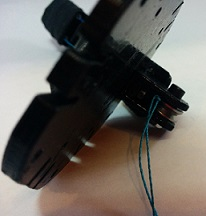
\includegraphics[width=5.5cm]{figures/Finger/TopPlate6.jpg}
    	\end{tabular}
  	\end{minipage}
};
\node[mytitle, right=10pt] at (box.north west) {6.6.2};
\end{tikzpicture}%
\end{center}

\vspace{0.1cm}

\begin{center}
\begin{tikzpicture}
\node [mybox] (box){%
  	\begin{minipage}[b]{0.50\linewidth}\centering
	\begin{tabular}{c }
		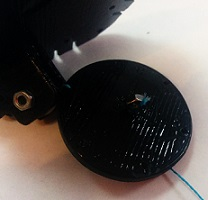
\includegraphics[width=5.5cm]{figures/Finger/TopPlate7.jpg}
    	\end{tabular}
	\end{minipage}
	\hspace{0.5cm}	
	\begin{minipage}[b]{0.50\linewidth}
	\begin{tabular}{ l }
		\Circled{1} Cut 400mm of Dyneema fishing line. \\
		\Circled{2} Pass the Dyneema from the hole of a M3 nut \\ and do a non-slip knot. \\
		\Circled{3} Insert the Dyneema into the centered hole \\ of the differential mechanism. \\
                \Circled{!} The nut will keep the Dyneema constrained \\ at the one side!
    	\end{tabular}
  	\end{minipage}
};
\node[mytitle, right=10pt] at (box.north west) {6.6.3};
\end{tikzpicture}%
\end{center}

\vspace{0.1cm}

\begin{center}
\begin{tikzpicture}
\node [mybox] (box){%
  	\begin{minipage}[b]{0.50\linewidth}\centering
	\begin{tabular}{ l }
		\Circled{1} Center the holes of the differential disk \\ with the TopPlate slots. \\ 
		\Circled{2} Insert one edge of the FingerBase Dyneema \\ into one of the holes of the differential. \\
		\Circled{3} With the two edges of the Dyneema do \\ multiple surgeon's knots. \\
		\Circled{4} Repeat the steps for all robot fingers. \\
    	\end{tabular}
	\end{minipage}
	\hspace{0.5cm}	
	\begin{minipage}[b]{0.50\linewidth}
	\begin{tabular}{ c }
		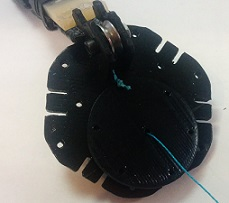
\includegraphics[width=5.5cm]{figures/Finger/TopPlate8.jpg}
    	\end{tabular}
  	\end{minipage}
};
\node[mytitle, right=10pt] at (box.north west) {6.6.4};
\end{tikzpicture}%
\end{center}